\section{Theory}

In this derivation, we will consider a photon of initial energy $E$ and momentum $p$ incident on a stationary electron of mass $m$. The photon is scattered at an angle $\theta$ with respect to its initial direction, and its final energy and momentum are $E^\prime$ and $p^\prime$, respectively.

We will begin by considering the conservation of energy and momentum in the Compton scattering process. The initial energy and momentum of the system are given by:

\begin{equation}
E + mc^2 = pc \label{eq1}
\end{equation}

where $c$ is the speed of light. After the scattering, the final energy and momentum of the system are given by:

\begin{equation}
E^\prime + \sqrt{p^{\prime 2}c^2 + m^2c^4} = p^\prime c \label{eq2}
\end{equation}

where the square root term represents the total energy of the electron after the scattering.

The energy and momentum of the photon before and after the scattering are given by:

\begin{align}
E &= \frac{hc}{\lambda} \label{eq3}\\
E^\prime &= \frac{hc}{\lambda^\prime} \label{eq4}
\end{align}

where $\lambda$ and $\lambda^\prime$ are the wavelengths of the photon before and after the scattering, respectively.

Using the conservation of energy and momentum, we can eliminate $E^\prime$ and $p^\prime$ in Eq.~(\ref{eq2}) to obtain:

\begin{equation}
\frac{hc}{\lambda^\prime} + \sqrt{p^{\prime 2}c^2 + m^2c^4} = (pc - p^\prime\cos\theta)c \label{eq5}
\end{equation}

where we have used the fact that the electron recoils in the direction opposite to the scattered photon, with a momentum of $p^\prime\cos\theta$.

Solving for $\lambda^\prime$ in Eq.~(\ref{eq5}), we obtain:

\begin{equation}
\lambda^\prime = \frac{h}{mc} \left(1 - \cos\theta + \frac{mc}{pc}(1 - \cos\theta)^2\right) \label{eq6}
\end{equation}

where we have used the fact that $p^{\prime 2}c^2 = E^{\prime 2} - m^2c^4$ and $E^\prime = hc/\lambda^\prime$.

We can simplify Eq.~(\ref{eq6}) by making use of the Compton wavelength of the electron, which is given by:

\begin{equation}
\lambda_c = \frac{h}{mc} \label{eq7}
\end{equation}

Substituting Eq.(\ref{eq7}) into Eq.(\ref{eq6}) yields:

\begin{equation}
\lambda^\prime - \lambda = \lambda_c (1 - \cos\theta) \label{eq8}
\end{equation}

which is the famous Compton formula.

Eq.~(\ref{eq8}) shows that the wavelength of the scattered photon is increased by an amount proportional to the Compton wavelength of the electron and the cosine of the scattering angle. This result can be interpreted as the photon transferring some of its energy and momentum to the electron, resulting in a decrease in the energy and frequency of the scattered photon.

\begin{figure}[htpb]
	\centering
	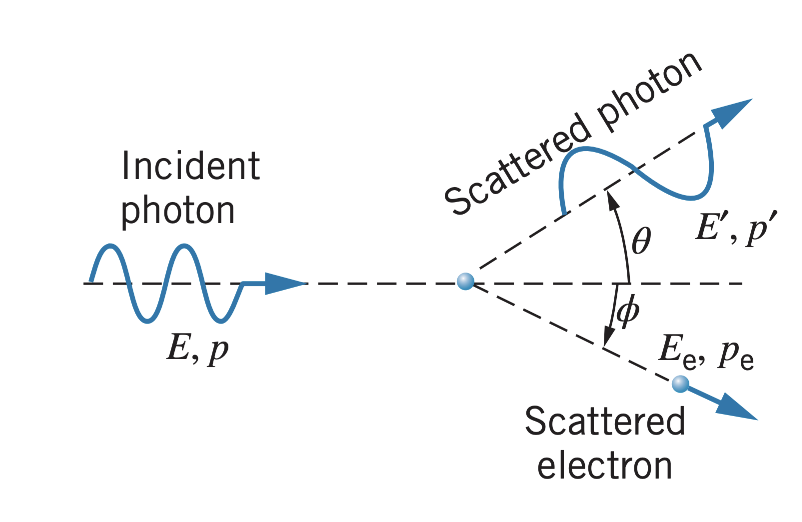
\includegraphics[width=0.4\textwidth]{figures/compton}
	\caption{A schematic diagram of compton process. (Krane, 2020)}
	\label{fig:figures-compton}
\end{figure}

In the Compton scattering experiment, we measure the energy and angle of the scattered photon. We can then test if the measured values satisfy Eq.~(\ref{eq8}). If the measured wavelength of the scattered photon is larger than the incident photon's wavelength, and the measured angle is consistent with the Compton formula, we can confirm that the Compton scattering process has occurred.

